\subsection{Фундаментальные понятия и принципы Квантовой Механики}

\subsubsection{Волны Де Бройля}

\begin{multicols}{2}
	
\paragraph{Общий случай} Плоская волна частотой $\omega$, распространяющаяся вдоль оси $x$:
\begin{equation*}
	\xi(x,t) = A \exp \left\{-i(\omega t -kx)\right\},
\end{equation*}
где $A$ - амплитуда, $k=\frac{2\pi}{\lambda}$ - волновое число.

\paragraph{Гипотеза Де Бройля} 
\thispagestyle{empty}
Свободной частице с энергией $E$ и импульсом $p$, движущейся вдоль $x$, соответсвует плоская волна:
\begin{equation*}
	\Psi(x, t) = A \exp \left\{-\frac{i}{\hbar}(E t - px)\right\}
\end{equation*}
Посмотрев на выражения волновых процессов в общем виде $\xi$ и для волны Де Бройля $\Psi$, заметим некоторые соотношения:
\begin{itemize}
	\item частота $\omega = \frac{E}{\hbar}$
	\item длина волны Де Бройля $\lambda_{\text{Б}}=\frac{2\pi\hbar}{p}$
	\item энергия $E = \hbar \omega = h\nu$
	\item $\vec p = \hbar \vec k$, где $\vec k$ - волновой вектор
\end{itemize}

\paragraph{Свойства волн Де Бройля}
\begin{enumerate}[label=\textbf{№~\arabic{enumi}}]
	\item В процессе распространения волны могут отражаться, преломляться, интерферировать и дифрагировать по обычным волновым законам
	
	\item Фазовая скорость $v_\text{фаз}$ - скорость, с которой распространяются точки волны с постоянной фазой.
	Выражение для фазовой скорости вытекает из условия постоянности фазы при его дифференцировании:
	\begin{equation*}
		Et-px=\mathrm{const} \overset{\dfrac{d}{dt}}{\longrightarrow} v_\text{фаз} = \frac{dx}{dt} = \frac{E}{p}.
	\end{equation*}
	При подстановке известных соотношений, а именно $E=mc^2$ и $p=mv$ в $v_\text{фаз}$, получим
	\begin{equation*}
		v_\text{фаз} = \frac{c^2}{v}
	\end{equation*} выражение для фазовой скорости\footnote{$v<c \implies v_\text{фаз} = \frac{c^2}{v} > c$ --- это не противоречит СТО. Ограничения, накладываемые СТО касаются скорости переноса массы/энергии, но фазовая скорость волны ничего из этого не характеризует.}.
	
	\item Групповая скорость $v_\text{гр}$
	\begin{equation*}
		v_\text{гр} = \frac{dw}{dk} = \frac{d(\hbar\omega)}{d(\hbar k)} = \frac{dE}{dp}
	\end{equation*}
	Возьмем известное всем выражение из теории относительности:
	\begin{equation*}
		E^2=p^2c^2+E_0^2=\left[E_0=m_0c^2\right]=E^2=p^2c^2+m_0^2c^4
	\end{equation*}
	Продифференцируем по t:
	\begin{equation*}
		2EdE=2pc^2dp\longrightarrow\frac{dE}{dp}=\frac{pc^2}{E}
	\end{equation*}
	Воспользовавшись этим знанием, получаем, что групповая скорость волны равна скорости движения частицы:
	\begin{equation*}
		v_\text{гр} = \frac{pc^2}{E} = \frac{pc^2}{mc^2} = \frac{p}{m} = v
	\end{equation*}
	
	\item Длина волны Де Бройля для нерелятивистских $(v\ll c)$ и релятивистких ($v\approx c$) частиц.
	\begin{itemize}
		\item Нерелятивисткий случай $(v\ll c)$:
		\begin{equation*}
		E_k=\frac{mv^2}{2}=\frac{p^2}{2m_0}\implies p=\sqrt{2m_0E_k}
		\end{equation*}
		\begin{equation*}
		\lambda_\text{Б}=\frac{2\pi\hbar}{p}=\frac{2\pi\hbar}{\sqrt{2m_0E_k}}
		\end{equation*}
		\item Релятивистский случай $(v\approx c)$:
		\begin{equation*}
		p=\frac{1}{c}\sqrt{E_k(E_k+2m_0c^2)} \Leftrightarrow
		\end{equation*}
		\begin{equation*}
		\Leftrightarrow p=\sqrt{2m_0E_k}\sqrt{1+\frac{E_k}{2m_0c^2}}
		\end{equation*}
		\begin{equation*}
			\lambda_\text{Б}'=\frac{2\pi\hbar}{p}=\frac{2\pi\hbar}{\sqrt{2m_0E_k}\sqrt{1+\frac{E_k}{2m_0c^2}}}
		\end{equation*}
		В этом выражении можно выделить нерелятивистскую дебройлевскую длину волны $\lambda_\text{Б}$, тогда 
		\begin{equation*}
			\lambda_\text{Б}'=\frac{\lambda_\text{Б}}{\sqrt{1+\frac{E_k}{2m_0c^2}}}
		\end{equation*}
	\end{itemize}
\end{enumerate}

\end{multicols}
\subsubsection{Соотношения неопределенностей Гейзенберга}
\begin{multicols}{2}
	\paragraph{Смысл}
	Двойственная корпускулярно-волновая природа микрочастиц накладывает ограничения на точность определения значений физических величин, характеризующих состояние частицы. Причем эти ограничения никак не связаны с точностью измерений, достижимой в конкретном эксперименте, а имеют принципиальное значение.
	\paragraph{Выражения для неопределенностей}
	\begin{equation*}
		\begin{cases}
		\left.\begin{array}{lll}
			\Delta p_x \Delta x & \geq \dfrac{\hbar}{2} &  \\[10pt]
			\Delta p_y \Delta y & \geq \dfrac{\hbar}{2} &  \\[10pt]
			\Delta p_z \Delta z & \geq \dfrac{\hbar}{2} &  
		\end{array}\right] \text{иногда пишут $\hbar$} \\[1.5cm]
		\begin{array}{rr}
			\Delta E \Delta t  & \geq \hbar 
		\end{array}
		\end{cases},
	\end{equation*}где $\Delta P_{x}$ --- неопределенность импульса $P_{x}$, \\
	$\Delta x$ --- неопределенность координаты $x$,\\
	$\Delta E$ --- неопределенность энергии,\\
	$\Delta t$ (иногда пишут $\tau$) --- среднее \textit{время жизни} в данном энергетическом состоянии.
	
	\paragraph{Общий ход вывода соотношений для моментов и координат}
	\begin{figure}[H]
		\centering
		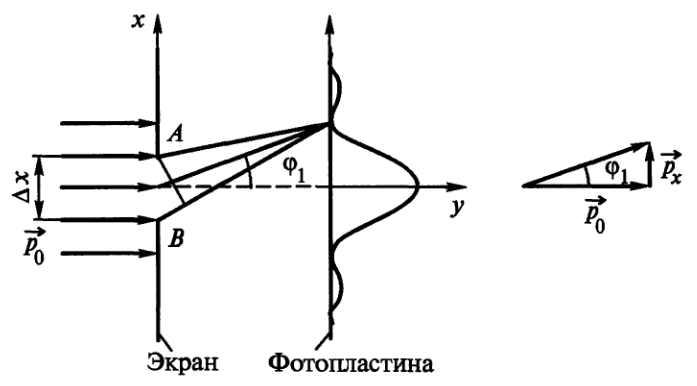
\includegraphics[width=.9\linewidth]{img/oral-01/electron-difraction}
		\caption{Картина дифракции электрона на щели}
		\label{fig:electron-difraction}
	\end{figure}
	(см Рис. \ref{fig:electron-difraction}) Пусть падающий электрон обладает импульсом $\vec p_0$. По гипотезе Де Бройля поставим в соответствие этому электрону плоскую волну с волновым вектором $\vec k = \frac{\vec p_0}{\hbar}$ и длиной волны $\lambda_{\text{Б}}=\frac{2\pi\hbar}{p_0}$.
	
	До прохождения щели известен импульс электрона $p_x=p_z=0,\, p_y=p_0$, а его координата $x$ неизвестна.
	
	При прохождении щели неопределенность координаты $x$ становится равной $\Delta x$, появляется неопределенность импульса $\Delta p_x$, обусловленная дифракцией электронов на щели\footnote{Электроны после прохождения щели описываются теперь не плоской, а расходящейся волной, интенсивность которой зависит от угла дифракции $\varphi$.}. Меняется также и проекция $p_x$ импульса электрона на ось $x$.
	
	Центральный дифракционный максимум, в который попадет большинство электронов, описывается углом $\varphi_1$, задающим первый минимум интенсивности. Из теории дифракции ($\Delta x \sin(\varphi_k)=k\lambda,\,k\in\mathbb{N}$) запишем уравнение для нахождения $\varphi_1,\,(k=1)$:
	\begin{equation*}
		\Delta x \sin \varphi_1=\lambda_{\text{Б}}
	\end{equation*}
	За счет малости $\varphi_1$ используем приближение:
	\begin{equation*}
		\frac{\lambda_{\text{Б}}}{\Delta x} = \sin \varphi_1 \approx \tg \varphi_1
	\end{equation*}
	В то же время угол $\varphi_1$ можно выразить через проекции $p_x,\,p_y$ импульса электрона:
	\begin{equation*}
		\tg \varphi_1 = \frac{p_x}{p_y} = \frac{p_x}{p_0}
	\end{equation*}
	Считая, что неопределенность $\Delta p_x$ сравнима с $p_x$, получаем:
	\begin{equation*}
		\tg \varphi_1 \approx \frac{\Delta p_x}{p_0}
	\end{equation*}
	Отсюда следует, что:
	\begin{equation*}
		\tg \varphi_1 \approx \frac{\Delta p_x}{p_0} \approx \frac{\lambda_{\text{Б}}}{\Delta x}
	\end{equation*}
	Окончательно получаем:
	\begin{equation*}
		\Delta x \Delta p_x \approx \lambda_{\text{Б}}p_0
	\end{equation*}
	Поскольку $\lambda_{\text{Б}}=\frac{2\pi\hbar}{p_0}$, то с учетом сделанных приближений и упрощений:
	\begin{equation*}
		\Delta x \Delta p_x \approx \underset{\text{пишут по разному}}{2\pi\hbar \geq \hbar \geq \frac{\hbar}{2}}
	\end{equation*}
	
	Поскольку ось $x$ физически ничем не была выделена, то аналогичное соотношение оказывается справедливым для других координатных осей $y$ и $z$.
\end{multicols}

\subsubsection{Постулаты квантовой механики}

\subsubsection{Принцип суперпозиции квантовых состояний}

\subsubsection{Принцип неразличимости тождественных частиц}
